\section{Model Training and Validation}
\label{sec:model_training}

\subsection{Training Dataset Generation}

Data distribution is a strong indicator of compressibility~\cite{devarajan2020hcompress}. To generate our compression training dataset, we developed a synthetic binned distribution generator that creates data with controlled statistical properties. The generator varies four key parameters: distribution type (uniform, normal, gamma, exponential), bin width (0, 1, 4, 8, 16 values), perturbation level (0 to 0.5, controlling run lengths), and data size (1 KB to 128 KB across 48 logarithmically-spaced values). Each generated chunk is compressed with all 29 library/configuration combinations across 11 compression libraries (BROTLI, BZIP2, Blosc2, FPZIP, LZ4, LZMA, SNAPPY, SZ3, ZFP, ZLIB, ZSTD) and three data types (char, int, float), resulting in 185,760 unique samples.

For each compression operation, we extract seven input features and four output targets. The input features are: library\_id (categorical), config\_id (categorical), datatype\_id (categorical), data\_size (bytes), shannon\_entropy (bits/byte), mean\_absolute\_deviation, and second\_order\_derivative (measuring data smoothness). The output targets are: compression\_ratio, compress\_time\_ms, decompress\_time\_ms, and psnr\_db (quality metric for lossy compression). The second-order derivative, computed as $\frac{1}{n-2}\sum_{i=1}^{n-2}|x_{i+1} - 2x_i + x_{i-1}|$, captures data curvature and proves to be the most important feature for predicting compression ratio, accounting for 49\% of predictive power.

\subsection{Model Training and Validation}

We conducted a hyperparameter study for the Q-table model, testing 64 configurations across four parameters. The number of bins for each continuous feature (data\_size, shannon\_entropy, mean\_absolute\_deviation) was tested at 5, 10, 15, and 20 bins, while the binning strategy was tested as either uniform (equal-width) or quantile (equal-frequency). Using 5-fold cross-validation, the optimal configuration was found to be 15 bins for size and entropy, 10 bins for MAD, with quantile binning. This configuration achieved a cross-validation R$^2$ of 0.74 with an unknown state rate of 7.3\% on the test set.

The Q-table training procedure discretizes continuous features into bins using the saved bin edges, constructs state tuples of the form (library\_id, config\_id, datatype\_id, size\_bin, entropy\_bin, mad\_bin, derivative\_bin), and computes the average target values for each unique state encountered during training. The resulting lookup table contains 33,155 unique states. For unknown states during inference, the model falls back to global averages, though this occurred for only 7.3\% of test samples.

\subsection{Model Architecture Comparison}

We compare three model architectures: XGBoost (gradient boosting), Q-table (tabular lookup), and DNN (multi-layer perceptron with 128-256-128-64 architecture). Figure~\ref{fig:r2_comparison} shows the R$^2$ scores for each model across all prediction targets. XGBoost achieves the highest accuracy overall (R$^2$ = 0.97), followed by Q-table (R$^2$ = 0.80) and DNN (R$^2$ = 0.66). XGBoost excels at all targets, particularly PSNR (R$^2$ = 0.999) and timing predictions (R$^2$ > 0.95). The Q-table performs well on timing predictions (compress time R$^2$ = 0.88, decompress time R$^2$ = 0.92) but shows lower accuracy for compression ratio (R$^2$ = 0.57). The DNN struggles with decompression time prediction (R$^2$ = 0.08) despite reasonable performance on other targets.

\begin{figure}[htbp]
\centering
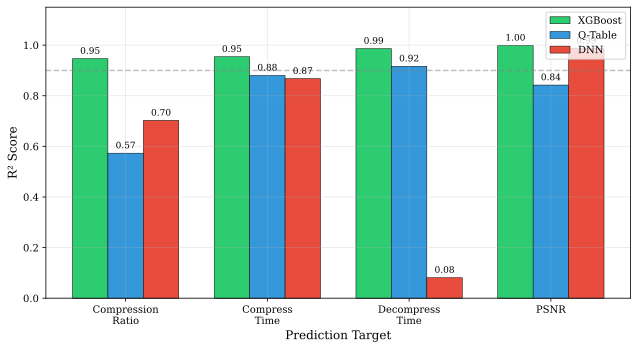
\includegraphics[width=0.9\textwidth]{r2_comparison.pdf}
\caption{R$^2$ score comparison across models and prediction targets. XGBoost achieves the highest accuracy for all targets, with particularly strong performance on compression ratio (0.95) and PSNR (0.999). The Q-table provides good accuracy for timing predictions but lower accuracy for compression ratio (0.57).}
\label{fig:r2_comparison}
\end{figure}

Figure~\ref{fig:inference_speed} compares inference latency, which is critical since prediction occurs on the I/O path. The C++ Q-table achieves 1.6 $\mu$s latency for predicting all 29 library/configuration combinations---272$\times$ faster than XGBoost (435 $\mu$s). For a typical 10ms compression operation, the Q-table adds only 0.02\% overhead versus 4.35\% for XGBoost. Given that our target application requires high-throughput compressor selection on the I/O path, we select the Q-table despite its lower R$^2$, as the speed advantage outweighs the accuracy tradeoff. The Q-table also supports online reinforcement learning for continuous adaptation to deployment-specific data characteristics.

\begin{figure}[htbp]
\centering
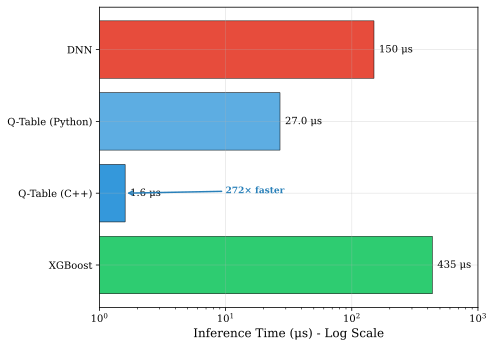
\includegraphics[width=0.85\textwidth]{inference_speed.pdf}
\caption{Inference speed comparison for predicting all 29 library/configuration combinations. The C++ Q-table achieves 1.6 $\mu$s latency (272$\times$ faster than XGBoost), making it suitable for high-throughput I/O paths where prediction overhead must be minimized.}
\label{fig:inference_speed}
\end{figure}
